\documentclass{article}
\usepackage[dblblindworkshop,nonatbib]{neurips_2026}
\usepackage[numbers,sort&compress]{natbib}

\usepackage[utf8]{inputenc}
\usepackage[T1]{fontenc}
\usepackage{hyperref}
\usepackage{url}
\usepackage{booktabs}
\usepackage{amsmath}
\usepackage{amssymb}
\usepackage{graphicx}

\title{Unreliability or Disagreement?\\
What an Interpercentile Decomposition Can and Cannot Show}

\workshoptitle{TAE (Trust-AI-Eval): Can We Trust AI Evaluation?}

\author{Anonymous Author(s)\\Affiliation\\\texttt{email}}

\usepackage{xcolor}
\ifdefined\answerYes\else\newcommand{\answerYes}[1][]{\textcolor{blue}{[Yes] #1}}\fi
\ifdefined\answerNo\else\newcommand{\answerNo}[1][]{\textcolor{orange}{[No] #1}}\fi
\ifdefined\answerNA\else\newcommand{\answerNA}[1][]{\textcolor{gray}{[NA] #1}}\fi

% inline math with both a superscript and a subscript raises line height;
% guarantee a visible gap rather than letting lines touch
\setlength{\lineskiplimit}{2pt}
\setlength{\lineskip}{2pt}

\begin{document}
\maketitle

\begin{abstract}
A widely cited result reports that language models ``get lost'' in multi-turn conversation, and
decomposes the degradation into a small loss of \emph{aptitude} and a large increase in
\emph{unreliability}, where aptitude is a high percentile of an instruction's score distribution
and unreliability is an interpercentile range. We show that this decomposition cannot support the interpretation usually placed on it. The underlying statistics are not new. Dispersion of a binary variable peaks at intermediate difficulty, a fact long known in classifier-ensemble diversity and item-response theory. They have not, however, been applied to this metric, and their consequences here are severe. Analytically: the two components are nested, since the range
is the difference of the two percentiles that define aptitude and the lower tail, so they are one
reparameterisation of a percentile pair rather than independent axes; at the original's own ten runs per instruction and under a binary scorer, the
range saturates at its maximum for seven of eleven possible outcomes and vanishes at both extremes, making it a near-binary indicator of whether an instruction is contested rather than a graded measure of reliability, so a
model that always fails is scored as reliably as one that always succeeds; and because a range is
non-negative, the comparison degenerates as a baseline saturates: the reported change is forced
non-negative in the limit, and its relative form is inflated well before that. Empirically, on 5{,}765 conversations we generated across seven models from six developers and three tasks, three of sixteen cells have a baseline unreliability of exactly zero, so
their headline increase is guaranteed by construction; a null containing no reliability parameter at all overproduces the original's headline unreliability rise while underproducing its aptitude drop, inverting the intended reading; and a binomial null that sees only
each cell's accuracies and run count, and nothing about the task, recovers the ordering of the
per-task results (Spearman $\rho = 0.66$). Replacing the statistic with an operational retry test separates what the decomposition conflates: on mathematics an oracle retry recovers $92\%$ of the degradation, while on function calling it recovers $48\%$ and leaves a gap strictly positive in seven of seven cells, with a fifth of instructions failing deterministically. We conclude that interpercentile decompositions should
be reported alongside the percentiles they are built from, and that benchmark saturation must be
checked before such a decomposition is interpreted.
\end{abstract}

\section{Introduction}

Empirical claims about language models are usually claims about a summary statistic. When that
statistic has structure the reader does not see, a conclusion can be an artefact of the
construction rather than a fact about models. This paper is a case study.

We take as our object of study the analysis of \citet{laban2025lost}, which reports that models
degrade sharply when an instruction is revealed over several turns rather than stated at once, and
decomposes that degradation into \emph{aptitude} $A_h$, the $h$th percentile of an instruction's
score distribution, and \emph{unreliability} $U^h_l = A_h - P_l$, the gap between the $h$th and
$l$th percentiles. The reported conclusion is that aptitude falls only slightly while unreliability
rises sharply, which invites the reading that models remain capable but become noisy.

The degradation itself is robust and we reproduce it in every condition we ran. Our contribution
concerns the \emph{decomposition}. We show that it cannot distinguish the interpretation it is
given from several alternatives, for reasons that are partly analytic and partly empirical, and we
quantify how much of an apparent per-task pattern survives a null model that knows nothing about
tasks.

\paragraph{Contributions.} (i) Three structural properties of the interpercentile decomposition:
nesting, non-monotonicity under coarse scorers, and degeneracy as a baseline saturates. (ii) A
reproduction on 5{,}765 self-generated conversations across seven models from six developers and three tasks,
showing all three properties bind in practice. (iii) A binomial null that recovers the ordering of
the per-task results without any task information, indicating that per-task differences in this
decomposition should not be read as facts about tasks.

\paragraph{Related work.} That the dispersion of a binary variable is maximal at intermediate
difficulty and vanishes at both extremes is long established. \citet{kuncheva2003diversity} define
the Kohavi--Wolpert variance for classifier ensembles with exactly this shape and tabulate
invariance under exchanging success and failure as a property of diversity measures;
\citet{gulliksen1945relation} makes the corresponding point for test items, and item-response
theory's information function has the same form. The standard remedy is to correct observed agreement against the agreement expected by chance at the observed base rate, as Fleiss's $\kappa$ does \citep{fleiss1971measuring}, and the associated base-rate paradoxes are well documented
\citep{feinstein1990high}. Closer to our setting, \citet{bowyer2025position} show that
normal-approximation intervals collapse spuriously as accuracy approaches zero or one in LLM
evaluation, and \citet{clark2023barda} note that a model can be trivially self-consistent by
answering uniformly. Our contribution is not the underlying statistics, which are textbook, but
their application to a specific and widely cited evaluation metric: what those facts imply for an
interpercentile decomposition, how severe the degeneracy is at the run counts actually used, and an
empirical demonstration on a reproduction. Evaluations elsewhere face the same pressure to fix an arbitrary analysis parameter: emergent-misalignment work gates generations on a coherence score with a threshold its authors call arbitrary, and then checks that the pattern of results survives varying it \citep{betley2025emergent}; downstream work adopts the same thresholds \citep{taylor2025school}. That is the practice we argue for, and it is what the decomposition we study lacks.

\section{Three properties of the decomposition}

Let an instruction be run $N$ times, giving scores $S = \{S_i\}_{i=1}^N$. Following
\citet{laban2025lost},
\begin{equation}
P \;=\; \mathrm{mean}(S), \qquad
A_h \;=\; \mathrm{percentile}_h(S), \qquad
U^h_l \;=\; \mathrm{percentile}_h(S) - \mathrm{percentile}_l(S) ,
\label{eq:defs}
\end{equation}
with deltas throughout being multi-turn minus single-turn. The original writes these as
$A^{90}$ and $U^{90}_{10}$; we keep $h$ and $l$ as free symbols so that the percentile
convention can be varied.

\paragraph{P1: the components are nested.} By definition $U^h_l = A_h - P_l$, so
$\Delta U = \Delta A - \Delta P_l$. Writing the contrast that the qualitative claim relies on as
$m = \Delta U - |\Delta A|$ and substituting, for any cell with $\Delta A \le 0$,
\begin{equation}
m \;=\; (\Delta A - \Delta P_l) + \Delta A \;=\; 2\,\Delta A - \Delta P_l .
\label{eq:identity}
\end{equation}
The comparison of ``unreliability against aptitude'' is therefore a comparison of the lower tail against twice the upper tail. The sharper statement is sufficiency: for $N$ exchangeable binary trials the success count is a sufficient statistic \citep{fisher1922mathematical}, so $A_h$, $P_l$, $U^h_l$, the mean and the variance are all deterministic functions of a single number, and no exchangeable summary of that sample can separate capability from consistency. It is one reparameterisation of the percentile pair
$(P_h, P_l)$, not two independent measurements, and a confidence interval on $\Delta A$ and one on
$\Delta U$ are not independent either. We verified Eq.~\ref{eq:identity} to numerical precision in
all 15 of our cells with $\Delta A \le 0$.

\paragraph{P2: under a coarse scorer, unreliability measures disagreement, not reliability.}
When the scorer is binary, $S$ is determined by the success count $k$, and so is $U^h_l$. The
original analysis uses $N = 10$ simulations per instruction, where $U^{90}_{10}$ takes the values
$0, 0.1, 1, 1, 1, 1, 1, 1, 1, 0.1, 0$ for $k = 0, \ldots, 10$: it is very nearly an
\emph{indicator} of whether between two and eight of the ten runs succeeded. At our $N = 6$ it is
$0, \tfrac12, 1, 1, 1, \tfrac12, 0$. So it saturates at its maximum across seven of the eleven possible outcomes, and $\mathbb{E}[U \mid p]$ is confined to $[0.863, 0.980]$ across the whole middle of the ability range. When $h + l = 1$ the statistic obeys $U(k) = U(N-k)$ exactly, so $\mathbb{E}[U \mid p]$ is symmetric about $p = 1/2$ and attains its maximum there: $\mathbb{E}[U \mid 0.3]$ and $\mathbb{E}[U \mid 0.7]$ are the same number, $0.8627$. It is therefore not merely low-resolution but non-monotone, and cannot even sign the direction of an ability change: a rise in $U$ is equally consistent with a model improving toward $p = 1/2$ or degrading toward it. In both cases it is \emph{non-monotone} and vanishes at $k = 0$ and $k = N$: a model that fails
every run is recorded as exactly as reliable as one that succeeds every run. Under a binary scorer
the reported doubling of ``unreliability'' therefore says that the share of \emph{contested}
instructions roughly doubled, which is a weaker and different statement. Figure~\ref{fig:metric}(b) shows $\mathbb{E}[U \mid p]$ under $\mathrm{Binomial}(N, p)$, an
inverted U peaking at $p = \tfrac12$. The statistic answers ``is this instruction contested?'',
which coincides with reliability only away from the extremes. Consequently $\Delta U$ is largely
determined by how far accuracy moves along that curve, and a model that degrades from perfect to
merely inconsistent and one that degrades from inconsistent to uniformly failing produce changes of
opposite sign for the same drop in accuracy. These values use linear interpolation between order statistics (the \textsc{numpy} default, Hyndman--Fan type~7); under an inverse-ECDF convention the saturation is wider still, covering eight of eleven outcomes. The obvious repair, rescaling the statistic by what is attainable at the observed base rate in the spirit of chance-corrected agreement coefficients \citep{fleiss1971measuring}, does not work here. For binary scores the plug-in ratio is $s^2 / (\hat{p}(1-\hat{p})) = N/(N-1)$ \emph{identically} for every $0 < k < N$, because the normaliser is a bijective function of the numerator. At $N = 10$ it equals $1.111$ for every outcome: base-rate normalisation does not restore resolution, it removes what little remained.

\paragraph{P3: as a baseline saturates, the comparison degenerates.} $U^h_l$ is a range, so
$U^h_l \ge 0$. In the limit where the baseline condition is saturated, $U^{\text{single}} = 0$ and
therefore $\Delta U = U^{\text{multi}} \ge 0$ whatever the model does: the metric cannot report a
reliability improvement even in principle, and the \emph{relative} change diverges. The original's
baselines are not at that limit: its single-turn unreliability is well away from zero, so its reported sign is not mechanically forced. Its relative form is nonetheless denominator-sensitive: the four of its models with the smallest single-turn unreliability show relative rises of $236\%$ to $285\%$, against a corpus-level $+112\%$ computed on means. It is our reproduction, not the original, that reaches the degenerate regime, with single-turn unreliability from $0.0$ to $20.4$ points against the original's $13$ to $49$. The authors note a related effect
for weak models, that lower Full scores leave ``less scope for degradation''
\citep{laban2025lost}, but treat it as a caveat about model comparison rather than about the
decomposition, and their limitations section raises no metric concern. Our reproduction reaches the
degenerate limit itself: three of sixteen cells have $U^{\text{single}}$ exactly zero.

\section{Setup}

The authors release sharded instructions but not their conversation logs, so all conversations here
were generated. Four of the original's six tasks are scored for binary correctness before being mapped onto a $0$--$100$ range \citep{laban2025lost}, so the coarse-scorer regime of P2 is the one its headline numbers largely occupy. We use three tasks with programmatic scorers, so that no model-graded judge enters
the pipeline: \emph{mathematics} (exact numeric match, 30 instructions), \emph{function calling}
(abstract-syntax-tree match, 25 instructions) and \emph{data-to-text} (BLEU against multiple
references, 25 instructions). Conversations were generated through a serverless inference API for
Llama~4 Maverick, Llama~3.3~70B, Qwen3-32B, DeepSeek~R1, Claude Sonnet~4.5, Mistral Pixtral Large
and Amazon Nova~2 Lite. The frozen corpus holds 7{,}048 lines, of which 7{,}047 parse and 6{,}794 carry a score (one line is truncated and is excluded);
5{,}765 conversations fall in the 16 model-task cells that pass our power gates.

Because $A_h$ and $U^h_l$ are percentiles taken \emph{within} an instruction, runs per instruction
is the binding constraint, not instruction count. We analyse a cell only if it has at least 10
instructions paired across both conditions and a median of at least 4 runs per instruction per
condition; 5 of 21 cells fail these gates and are excluded and listed, not silently dropped. Both
conditions are always evaluated on an identical instruction set. Confidence intervals are bootstrap
intervals over instructions ($B = 2000$).

\section{Results}

\paragraph{The degradation reproduces.} Multi-turn performance falls in every cell, by $-5.9$ to
$-65.3$ percentage points. We do not dispute the original headline finding.

\paragraph{Aptitude is a threshold readout, not a capability measure.} The same reduction applies to $A_h$. At $N = 10$, $\mathbb{E}[A_{90} \mid p]$ crosses $1/2$ at $p = 0.153$ and exceeds $0.998$ for every $p \ge 0.6$: it is a smoothed indicator of $p > 0.15$, with no resolution across the range where capable models operate. Aptitude and unreliability are thus two threshold readouts of one instruction-difficulty distribution, taken at different cut points, rather than two axes of model behaviour.

\paragraph{A null with no reliability parameter overproduces the headline effect.} We can ask
directly how much of the reported pattern survives removing reliability from the data-generating
process. Draw per-instruction success probabilities $p_i \sim \mathrm{Beta}$ calibrated to a single-turn accuracy near ceiling and a multi-turn drop of comparable size to the original's reported degradation, and let the $N$ runs of an
instruction be independent $\mathrm{Bernoulli}(p_i)$. This model has no reliability parameter at
all: every run is exchangeable and independent given the instruction. Across concentrations from 2
to 30 it yields $\Delta U$ between $+167\%$ and $+196\%$, against the reported $+112\%$, and $\Delta A$ between $-0.2\%$ and $-6.9\%$, against the reported $-16\%$. The reported rise in
unreliability is therefore \emph{smaller} than a model with no reliability structure produces, while
the reported fall in aptitude is \emph{larger}. Read against the right null, the anomalous component
of the degradation is the loss of capability, not the growth of variance, which is the opposite of the
conclusion the decomposition is used to support.

\paragraph{Read correctly, the original's own statistic shows capability collapse.} Because $\mathbb{E}[A_h \mid p]$ is increasing, for any difficulty distribution $G$ and any $t$ we have the distribution-free bound $G([0,t]) \ge \Phi_A(t) - \bar{A}$, where $\Phi_A$ is the transfer function above. The original reports a $16\%$ relative fall in aptitude, so its multi-turn $\bar{A} \le 0.84$. The bound then forces at least $15\%$ of instructions below a multi-turn success probability of $0.5$, and at least $16\%$ below $0.7$. That is a hard capability loss on a sixth of the instruction set, derived from the very statistic offered as evidence that capability was largely preserved.

\paragraph{The degenerate limit is reached in practice.} Table~\ref{tab:main} reports each cell's baseline unreliability
$U^{\text{single}}$ alongside the decomposition. Seven of sixteen cells have
$U^{\text{single}} < 5$pp, and in all seven $\Delta U > 0$. In three cells $U^{\text{single}}$ is
\emph{exactly} zero, so their reported increases of $+20.0$, $+30.0$ and $+44.4$ points are
non-negative by construction and carry no evidence about reliability.

\paragraph{The original's relative claim is more robust than its absolute form.} The original
reports \emph{relative} changes (aptitude $-16\%$, unreliability $+112\%$). Because
$U^{\text{single}}$ is small whenever the baseline is near ceiling, a small absolute rise in a
small denominator yields a large percentage. Evaluated in relative form, the ordering holds in
14 of our 16 cells, against 10 of 16 in absolute form. The relative statement is thus better
supported, but it is also the form most inflated by a saturated baseline, so the two
parameterisations should be reported together.

\paragraph{A task-blind null recovers the per-task ordering.} If one groups cells by task, the
contrast $m$ has median $+23.3$ on mathematics, $+0.0$ on function calling and $-8.5$ on
data-to-text, which invites a claim that the decomposition is task-dependent. We test that against
a null in which each cell is a homogeneous binomial with only that cell's single-turn and
multi-turn accuracy and its run count, and no information about the task. The null reproduces the
ordering of the observed margins (Spearman $\rho = 0.66$, Figure~\ref{fig:metric}(c)), while badly
misestimating their magnitudes, as expected since real instructions are heterogeneous. The
qualitative per-task pattern is therefore substantially recoverable from accuracy and run count
alone, and should not be read as a fact about tasks.

\begin{table}[t]
\centering
\caption{Decomposition at the $90/10$ convention on our frozen corpus. $U^{\mathrm{s}}$ is
single-turn unreliability. Cells with $U^{\mathrm{s}} = 0$ (marked $\dagger$) have
$\Delta U \ge 0$ by construction. $m = \Delta U - |\Delta A|$.}
\label{tab:main}
\small
\begin{tabular}{llrrrrr}
\toprule
Task & Model & $U^{\mathrm{s}}$ & $\Delta P$ & $\Delta A$ & $\Delta U$ & $m$\\
\midrule
Mathematics & Llama 4 Maverick & $10.0$ & $-35.0$ & $-10.3$ & $+37.7$ & $+27.3$\\
Mathematics & Nova 2 Lite & $6.7$ & $-37.1$ & $-15.0$ & $+40.7$ & $+25.7$\\
Mathematics & Qwen3-32B & $16.3$ & $-33.6$ & $-18.0$ & $+41.3$ & $+23.3$\\
Mathematics & DeepSeek R1 & $6.7$ & $-28.6$ & $-10.3$ & $+33.3$ & $+23.0$\\
Mathematics & Claude Sonnet 4.5 & $1.7$ & $-26.2$ & $-13.3$ & $+26.7$ & $+13.3$\\
\midrule
Function calling & Nova 2 Lite & $0.0$$^\dagger$ & $-53.1$ & $-32.0$ & $+44.4$ & $+12.4$\\
Function calling & Qwen3-32B & $2.0$ & $-46.8$ & $-30.0$ & $+36.4$ & $+6.4$\\
Function calling & Llama 4 Maverick & $0.0$$^\dagger$ & $-39.3$ & $-26.0$ & $+30.0$ & $+4.0$\\
Function calling & Llama 3.3 70B & $0.0$$^\dagger$ & $-30.7$ & $-20.0$ & $+20.0$ & $+0.0$\\
Function calling & DeepSeek R1 & $2.0$ & $-65.3$ & $-45.6$ & $+38.8$ & $-6.8$\\
Function calling & Claude Sonnet 4.5 & $5.3$ & $-41.0$ & $-29.5$ & $+22.1$ & $-7.4$\\
Function calling & Mistral Pixtral L & $20.0$ & $-32.8$ & $-27.6$ & $+9.5$ & $-18.1$\\
\midrule
Data-to-text & Llama 4 Maverick & $9.4$ & $-5.9$ & $+0.1$ & $+11.7$ & $+11.6$\\
Data-to-text & Llama 3.3 70B & $5.3$ & $-13.9$ & $-10.6$ & $+5.8$ & $-4.8$\\
Data-to-text & DeepSeek R1 & $14.4$ & $-10.2$ & $-10.9$ & $-1.4$ & $-12.3$\\
Data-to-text & Qwen3-32B & $17.3$ & $-9.4$ & $-11.0$ & $-3.3$ & $-14.4$\\
\bottomrule
\end{tabular}
\end{table}

\begin{figure}[t]
\centering
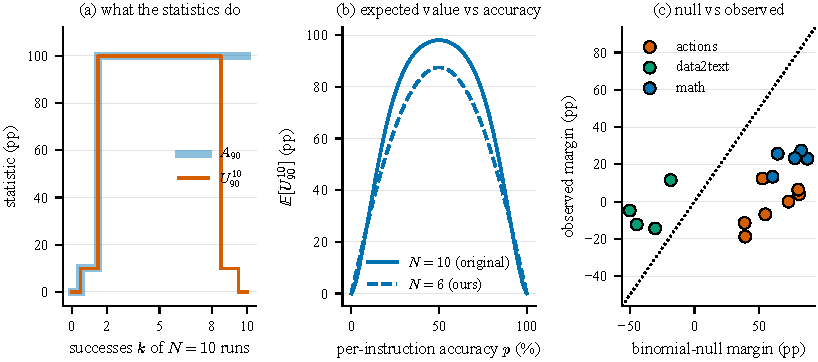
\includegraphics[width=\textwidth]{figM1_metric.pdf}
\caption{(a) With a binary scorer at the original's $N=10$, both statistics are step
functions of the success count $k$: $A_{90}$ is a threshold indicator, and $U^{90}_{10}$ saturates
at its maximum for $k = 2 \ldots 8$ and vanishes at both ends, so a model that always fails scores
as reliably as one that always succeeds. (b) Expected unreliability against per-instruction accuracy
at $N=10$ (solid) and our $N=6$ (dashed); it is non-monotone and symmetric about $p = 1/2$.
(c) Observed per-cell contrast $m$ against a binomial null using only each cell's accuracies and run
count, with no task information; the dotted line is equality. The null recovers the ordering
($\rho = 0.66$) while misestimating magnitudes.}
\label{fig:metric}
\end{figure}

\begin{table}[t]
\centering
\caption{Operational retry test. Gap is single-turn minus multi-turn mean score. Recovered is the
share of that gap closed by an \emph{oracle} best-of-$K$ over the multi-turn runs, which
upper-bounds any deployable strategy. Unrecoverable is the residual gap in instructions solved at
least once single-turn but never multi-turn, with a bootstrap interval over instructions;
$^{\ast}$ marks intervals strictly above zero. Deterministic failures are solved in \emph{every}
single-turn run and in \emph{no} multi-turn run.}
\label{tab:retry}
\small
\begin{tabular}{llrrrcr}
\toprule
Task & Model & Gap & Recov.\ (\%) & Unrec.\ (pp) & 95\% CI & Determ.\ (\%)\\
\midrule
Mathematics & Llama 4 Maverick & $35.0$ & $108.2$ & $3.3$ & $[0.0, 10.0]$ & $0.0$\\
Mathematics & DeepSeek R1 & $28.6$ & $98.5$ & $3.3$ & $[0.0, 10.0]$ & $3.3$\\
Mathematics & Qwen3-32B & $33.6$ & $91.8$ & $10.0$ & $[0.0, 23.3]$ & $3.3$\\
Mathematics & Nova 2 Lite & $37.1$ & $80.5$ & $10.0$ & $[-3.3, 23.3]$ & $10.0$\\
Mathematics & Claude Sonnet 4.5 & $26.2$ & $64.0$ & $10.0$ & $[-3.3, 23.3]$ & $13.3$\\
\midrule
Function calling & Qwen3-32B & $46.8$ & $58.7$ & $20.0$$^{\ast}$ & $[7.9, 36.0]$ & $20.0$\\
Function calling & Mistral Pixtral L & $32.8$ & $53.8$ & $23.8$$^{\ast}$ & $[9.5, 42.9]$ & $14.3$\\
Function calling & Llama 4 Maverick & $39.3$ & $49.2$ & $20.0$$^{\ast}$ & $[4.0, 36.0]$ & $20.0$\\
Function calling & Llama 3.3 70B & $30.7$ & $47.8$ & $16.0$$^{\ast}$ & $[4.0, 32.0]$ & $16.0$\\
Function calling & Nova 2 Lite & $53.1$ & $47.2$ & $28.0$$^{\ast}$ & $[8.0, 48.0]$ & $32.0$\\
Function calling & DeepSeek R1 & $65.3$ & $45.9$ & $36.0$$^{\ast}$ & $[16.0, 56.0]$ & $36.0$\\
Function calling & Claude Sonnet 4.5 & $41.0$ & $40.0$ & $26.3$$^{\ast}$ & $[5.3, 47.4]$ & $26.3$\\
\bottomrule
\end{tabular}
\end{table}

\paragraph{An operational test: is the loss actually recoverable?} The decomposition's practical
promise is falsifiable. If capability is intact and only consistency is lost, then \emph{retrying}
should recover the loss. We test this directly, counting an instruction as solved under a condition
if at least one of its runs succeeds. This is an oracle: it assumes a perfect verifier that can pick
the successful attempt, so it upper-bounds anything a deployment could achieve.

On mathematics the promise holds (Table~\ref{tab:retry}). Oracle retry recovers a median $91.8\%$ of the single-to-multi
gap across five models, and the residual unrecoverable gap of $10.0$ points has a bootstrap
interval covering zero in five of five cells. Multi-turn mathematics really is a consistency
problem.

On function calling it fails. Oracle retry recovers only $47.8\%$ of the gap, and the unrecoverable
remainder is $23.8$ points with a bootstrap interval strictly above zero in \emph{seven of seven}
cells. A median $20.0\%$ of instructions are \emph{deterministic} failures: solved in every
single-turn run and in none of the multi-turn runs. No number of retries recovers them, because
there is nothing inconsistent about them: the capability is simply absent once the instruction is
sharded.

This is the distinction the decomposition is used to make, and it is the distinction it cannot make.
Both task families show a large drop in $P$ and a large rise in $U$; only the retry test separates
the case where capability survives from the case where it does not. It also costs nothing extra: it
reuses the same runs, and unlike $U^h_l$ it is monotone in capability, has an unambiguous estimand,
and states a quantity a practitioner can act on.

\section{Discussion}

None of this shows that models do not degrade in multi-turn conversation. They do, in every cell we
ran, and that finding is not in question. What the decomposition cannot do is license the reading
that capability is preserved while reliability falls. By P1 the two quantities are one
reparameterisation of a percentile pair; by P2 the reliability term is a disagreement rate that
falls to zero when a model fails consistently; and by P3 its reported direction is fixed in advance
whenever the baseline is saturated, which our data show is the common case.

The practical stake is not rhetorical. A practitioner told that models are ``as capable but less
reliable'' will reach for sampling or self-consistency. In our function-calling cells, aptitude
falls by 20 to 46 points, so best-case capability is genuinely lost and repeated sampling addresses
the smaller part of the problem.

\paragraph{Recommendations.} Report $P_h$ and $P_l$ directly alongside any interpercentile range;
report the baseline value of the range, since a reader cannot otherwise tell a forced sign from an
informative one; state the percentile convention and the number of runs per item, both of which set
the resolution of the estimate; prefer a scorer with more than two levels when the object of study is variability; and do not expect base-rate normalisation to repair a within-instruction dispersion statistic, since for binary scores it is constant. A consistency claim needs either graded scores with at least three levels, a second replication factor against which extra-binomial variation can be tested, or an order-dependent statistic.

\paragraph{Limitations.} Our tasks use three different scorer types, so per-task magnitudes are not
comparable across tasks; this is one reason we argue the per-task reading is unsafe rather than
proposing a corrected per-task claim. Our data-to-text condition does not invoke the LLM
user-simulator, so it carries no simulator variance, unlike the other two tasks. Most cells use six
runs per instruction, which places $A_{90}$ and $U^{90}_{10}$ on a three-point lattice under a
binary scorer and limits per-cell resolution to $50/M$ points for $M$ instructions; margins should
be read at that resolution. We study open-weight and API models different from the original, so
absolute levels are not comparable to it. The binomial null is a homogeneous approximation and is
offered as a check on the per-task reading, not as a model of the data.

\paragraph{Data and reproducibility.} The frozen corpus of 7{,}048 records, the analysis scripts and
a README with the exact regeneration commands are released as supplementary material. All numbers
here come from that frozen snapshot.

\bibliographystyle{plainnat}
\begin{thebibliography}{99}
\bibitem[Betley et al.(2025)]{betley2025emergent} J.~Betley, D.~Tan, N.~Warncke,
A.~Sztyber-Betley, X.~Bao, M.~Soto, N.~Labenz, and O.~Evans. Emergent misalignment: narrow
finetuning can produce broadly misaligned LLMs. \emph{ICML}, 2025. arXiv:2502.17424. Extended
version in \emph{Nature}, 2026, doi:10.1038/s41586-025-09937-5.
\bibitem[Bowyer et al.(2025)]{bowyer2025position} S.~Bowyer, L.~Aitchison, and D.~R.~Ivanova.
Position: Don't use the CLT in LLM evals with fewer than a few hundred datapoints. \emph{ICML},
2025. arXiv:2503.01747.
\bibitem[Clark et al.(2023)]{clark2023barda} P.~Clark, B.~Dalvi Mishra, and O.~Tafjord. BaRDa: a
belief and reasoning dataset that separates factual accuracy and reasoning ability.
\emph{arXiv:2312.07527}, 2023.
\bibitem[Feinstein and Cicchetti(1990)]{feinstein1990high} A.~R.~Feinstein and D.~V.~Cicchetti.
High agreement but low kappa: I. the problems of two paradoxes. \emph{Journal of Clinical
Epidemiology}, 43(6):543--549, 1990.
\bibitem[Fisher(1922)]{fisher1922mathematical} R.~A.~Fisher. On the mathematical foundations of
theoretical statistics. \emph{Philosophical Transactions of the Royal Society A}, 222:309--368,
1922.
\bibitem[Fleiss(1971)]{fleiss1971measuring} J.~L.~Fleiss. Measuring nominal scale agreement among
many raters. \emph{Psychological Bulletin}, 76(5):378--382, 1971.
\bibitem[Gulliksen(1945)]{gulliksen1945relation} H.~Gulliksen. The relation of item difficulty and
inter-item correlation to test variance and reliability. \emph{Psychometrika}, 10(2):79--91, 1945.
\bibitem[Kuncheva and Whitaker(2003)]{kuncheva2003diversity} L.~I.~Kuncheva and C.~J.~Whitaker.
Measures of diversity in classifier ensembles and their relationship with the ensemble accuracy.
\emph{Machine Learning}, 51:181--207, 2003.
\bibitem[Laban et al.(2025)]{laban2025lost} P.~Laban, H.~Hayashi, Y.~Zhou, and J.~Neville. LLMs get
lost in multi-turn conversation. \emph{arXiv:2505.06120}, 2025.
\bibitem[Taylor et al.(2025)]{taylor2025school} M.~Taylor, J.~Chua, J.~Betley, J.~Treutlein,
and O.~Evans. School of reward hacks: hacking harmless tasks generalizes to misaligned
behavior in LLMs. \emph{arXiv:2508.17511}, 2025.
\end{thebibliography}

\newpage
\section*{NeurIPS Paper Checklist}

\begin{enumerate}

\item {\bf Claims}
    \item[] Question: Do the main claims made in the abstract and introduction accurately reflect the paper's contributions and scope?
    \item[] Answer: \answerYes{}
    \item[] Justification: The abstract and introduction claim a reproduction of the degradation and task-dependence of its decomposition, which is exactly what the results report, including the cells where the original characterisation holds.
    \item[] Guidelines:
    \begin{itemize}
        \item The answer \answerNA{} means that the abstract and introduction do not include the claims made in the paper.
        \item The abstract and/or introduction should clearly state the claims made, including the contributions made in the paper and important assumptions and limitations. A \answerNo{} or \answerNA{} answer to this question will not be perceived well by the reviewers. 
        \item The claims made should match theoretical and experimental results, and reflect how much the results can be expected to generalize to other settings. 
        \item It is fine to include aspirational goals as motivation as long as it is clear that these goals are not attained by the paper. 
    \end{itemize}

\item {\bf Limitations}
    \item[] Question: Does the paper discuss the limitations of the work performed by the authors?
    \item[] Answer: \answerYes{}
    \item[] Justification: A dedicated Limitations paragraph discusses scorer heterogeneity across tasks, the mix of open-weight and API models, the absence of simulator variance in one task, and the coarse percentile resolution at six runs per instruction.
    \item[] Guidelines:
    \begin{itemize}
        \item The answer \answerNA{} means that the paper has no limitation while the answer \answerNo{} means that the paper has limitations, but those are not discussed in the paper. 
        \item The authors are encouraged to create a separate ``Limitations'' section in their paper.
        \item The paper should point out any strong assumptions and how robust the results are to violations of these assumptions (e.g., independence assumptions, noiseless settings, model well-specification, asymptotic approximations only holding locally). The authors should reflect on how these assumptions might be violated in practice and what the implications would be.
        \item The authors should reflect on the scope of the claims made, e.g., if the approach was only tested on a few datasets or with a few runs. In general, empirical results often depend on implicit assumptions, which should be articulated.
        \item The authors should reflect on the factors that influence the performance of the approach. For example, a facial recognition algorithm may perform poorly when image resolution is low or images are taken in low lighting. Or a speech-to-text system might not be used reliably to provide closed captions for online lectures because it fails to handle technical jargon.
        \item The authors should discuss the computational efficiency of the proposed algorithms and how they scale with dataset size.
        \item If applicable, the authors should discuss possible limitations of their approach to address problems of privacy and fairness.
        \item While the authors might fear that complete honesty about limitations might be used by reviewers as grounds for rejection, a worse outcome might be that reviewers discover limitations that aren't acknowledged in the paper. The authors should use their best judgment and recognize that individual actions in favor of transparency play an important role in developing norms that preserve the integrity of the community. Reviewers will be specifically instructed to not penalize honesty concerning limitations.
    \end{itemize}

\item {\bf Theory assumptions and proofs}
    \item[] Question: For each theoretical result, does the paper provide the full set of assumptions and a complete (and correct) proof?
    \item[] Answer: \answerNA{}
    \item[] Justification: The paper contains no theoretical results; the monotonicity observation about coupled percentile quantities is arithmetic, not a theorem.
    \item[] Guidelines:
    \begin{itemize}
        \item The answer \answerNA{} means that the paper does not include theoretical results. 
        \item All the theorems, formulas, and proofs in the paper should be numbered and cross-referenced.
        \item All assumptions should be clearly stated or referenced in the statement of any theorems.
        \item The proofs can either appear in the main paper or the supplemental material, but if they appear in the supplemental material, the authors are encouraged to provide a short proof sketch to provide intuition. 
        \item Inversely, any informal proof provided in the core of the paper should be complemented by formal proofs provided in appendix or supplemental material.
        \item Theorems and Lemmas that the proof relies upon should be properly referenced. 
    \end{itemize}

    \item {\bf Experimental result reproducibility}
    \item[] Question: Does the paper fully disclose all the information needed to reproduce the main experimental results of the paper to the extent that it affects the main claims and/or conclusions of the paper (regardless of whether the code and data are provided or not)?
    \item[] Answer: \answerYes{}
    \item[] Justification: The Setup section specifies tasks, scorers, instruction counts, runs per condition, models, decomposition definitions and conventions; the simulation harness is the original authors' public code.
    \item[] Guidelines:
    \begin{itemize}
        \item The answer \answerNA{} means that the paper does not include experiments.
        \item If the paper includes experiments, a \answerNo{} answer to this question will not be perceived well by the reviewers: Making the paper reproducible is important, regardless of whether the code and data are provided or not.
        \item If the contribution is a dataset and\slash or model, the authors should describe the steps taken to make their results reproducible or verifiable. 
        \item Depending on the contribution, reproducibility can be accomplished in various ways. For example, if the contribution is a novel architecture, describing the architecture fully might suffice, or if the contribution is a specific model and empirical evaluation, it may be necessary to either make it possible for others to replicate the model with the same dataset, or provide access to the model. In general. releasing code and data is often one good way to accomplish this, but reproducibility can also be provided via detailed instructions for how to replicate the results, access to a hosted model (e.g., in the case of a large language model), releasing of a model checkpoint, or other means that are appropriate to the research performed.
        \item While NeurIPS does not require releasing code, the conference does require all submissions to provide some reasonable avenue for reproducibility, which may depend on the nature of the contribution. For example
        \begin{enumerate}
            \item If the contribution is primarily a new algorithm, the paper should make it clear how to reproduce that algorithm.
            \item If the contribution is primarily a new model architecture, the paper should describe the architecture clearly and fully.
            \item If the contribution is a new model (e.g., a large language model), then there should either be a way to access this model for reproducing the results or a way to reproduce the model (e.g., with an open-source dataset or instructions for how to construct the dataset).
            \item We recognize that reproducibility may be tricky in some cases, in which case authors are welcome to describe the particular way they provide for reproducibility. In the case of closed-source models, it may be that access to the model is limited in some way (e.g., to registered users), but it should be possible for other researchers to have some path to reproducing or verifying the results.
        \end{enumerate}
    \end{itemize}


\item {\bf Open access to data and code}
    \item[] Question: Does the paper provide open access to the data and code, with sufficient instructions to faithfully reproduce the main experimental results, as described in supplemental material?
    \item[] Answer: \answerYes{}
    \item[] Justification: All scored conversation logs and analysis scripts are released as supplementary material, as stated in the data and reproducibility paragraph.
    \item[] Guidelines:
    \begin{itemize}
        \item The answer \answerNA{} means that paper does not include experiments requiring code.
        \item Please see the NeurIPS code and data submission guidelines (\url{https://neurips.cc/public/guides/CodeSubmissionPolicy}) for more details.
        \item While we encourage the release of code and data, we understand that this might not be possible, so \answerNo{} is an acceptable answer. Papers cannot be rejected simply for not including code, unless this is central to the contribution (e.g., for a new open-source benchmark).
        \item The instructions should contain the exact command and environment needed to run to reproduce the results. See the NeurIPS code and data submission guidelines (\url{https://neurips.cc/public/guides/CodeSubmissionPolicy}) for more details.
        \item The authors should provide instructions on data access and preparation, including how to access the raw data, preprocessed data, intermediate data, and generated data, etc.
        \item The authors should provide scripts to reproduce all experimental results for the new proposed method and baselines. If only a subset of experiments are reproducible, they should state which ones are omitted from the script and why.
        \item At submission time, to preserve anonymity, the authors should release anonymized versions (if applicable).
        \item Providing as much information as possible in supplemental material (appended to the paper) is recommended, but including URLs to data and code is permitted.
    \end{itemize}


\item {\bf Experimental setting/details}
    \item[] Question: Does the paper specify all the training and test details (e.g., data splits, hyperparameters, how they were chosen, type of optimizer) necessary to understand the results?
    \item[] Answer: \answerYes{}
    \item[] Justification: No models are trained. All inference settings (sampling counts, conversation protocol, scorer definitions) are given in the Setup section.
    \item[] Guidelines:
    \begin{itemize}
        \item The answer \answerNA{} means that the paper does not include experiments.
        \item The experimental setting should be presented in the core of the paper to a level of detail that is necessary to appreciate the results and make sense of them.
        \item The full details can be provided either with the code, in appendix, or as supplemental material.
    \end{itemize}

\item {\bf Experiment statistical significance}
    \item[] Question: Does the paper report error bars suitably and correctly defined or other appropriate information about the statistical significance of the experiments?
    \item[] Answer: \answerYes{}
    \item[] Justification: The retry table reports bootstrap confidence intervals resampled over instructions (B=2000), the unit at which conditions are paired. Table 1 reports point estimates only; its intervals are included in the released results file.
    \item[] Guidelines:
    \begin{itemize}
        \item The answer \answerNA{} means that the paper does not include experiments.
        \item The authors should answer \answerYes{} if the results are accompanied by error bars, confidence intervals, or statistical significance tests, at least for the experiments that support the main claims of the paper.
        \item The factors of variability that the error bars are capturing should be clearly stated (for example, train/test split, initialization, random drawing of some parameter, or overall run with given experimental conditions).
        \item The method for calculating the error bars should be explained (closed form formula, call to a library function, bootstrap, etc.)
        \item The assumptions made should be given (e.g., Normally distributed errors).
        \item It should be clear whether the error bar is the standard deviation or the standard error of the mean.
        \item It is OK to report 1-sigma error bars, but one should state it. The authors should preferably report a 2-sigma error bar than state that they have a 96\% CI, if the hypothesis of Normality of errors is not verified.
        \item For asymmetric distributions, the authors should be careful not to show in tables or figures symmetric error bars that would yield results that are out of range (e.g., negative error rates).
        \item If error bars are reported in tables or plots, the authors should explain in the text how they were calculated and reference the corresponding figures or tables in the text.
    \end{itemize}

\item {\bf Experiments compute resources}
    \item[] Question: For each experiment, does the paper provide sufficient information on the computer resources (type of compute workers, memory, time of execution) needed to reproduce the experiments?
    \item[] Answer: \answerYes{}
    \item[] Justification: All inference ran through a commercial serverless inference API; no local GPUs were used. Total volume is the conversation counts reported per cell.
    \item[] Guidelines:
    \begin{itemize}
        \item The answer \answerNA{} means that the paper does not include experiments.
        \item The paper should indicate the type of compute workers CPU or GPU, internal cluster, or cloud provider, including relevant memory and storage.
        \item The paper should provide the amount of compute required for each of the individual experimental runs as well as estimate the total compute. 
        \item The paper should disclose whether the full research project required more compute than the experiments reported in the paper (e.g., preliminary or failed experiments that didn't make it into the paper). 
    \end{itemize}
    
\item {\bf Code of ethics}
    \item[] Question: Does the research conducted in the paper conform, in every respect, with the NeurIPS Code of Ethics \url{https://neurips.cc/public/EthicsGuidelines}?
    \item[] Answer: \answerYes{}
    \item[] Justification: The work re-analyses published benchmark tasks with API-served models and conforms to the Code of Ethics.
    \item[] Guidelines:
    \begin{itemize}
        \item The answer \answerNA{} means that the authors have not reviewed the NeurIPS Code of Ethics.
        \item If the authors answer \answerNo, they should explain the special circumstances that require a deviation from the Code of Ethics.
        \item The authors should make sure to preserve anonymity (e.g., if there is a special consideration due to laws or regulations in their jurisdiction).
    \end{itemize}


\item {\bf Broader impacts}
    \item[] Question: Does the paper discuss both potential positive societal impacts and negative societal impacts of the work performed?
    \item[] Answer: \answerNA{}
    \item[] Justification: This is a methodological reproduction about evaluation reporting; it has no direct deployment pathway beyond encouraging convention disclosure.
    \item[] Guidelines:
    \begin{itemize}
        \item The answer \answerNA{} means that there is no societal impact of the work performed.
        \item If the authors answer \answerNA{} or \answerNo, they should explain why their work has no societal impact or why the paper does not address societal impact.
        \item Examples of negative societal impacts include potential malicious or unintended uses (e.g., disinformation, generating fake profiles, surveillance), fairness considerations (e.g., deployment of technologies that could make decisions that unfairly impact specific groups), privacy considerations, and security considerations.
        \item The conference expects that many papers will be foundational research and not tied to particular applications, let alone deployments. However, if there is a direct path to any negative applications, the authors should point it out. For example, it is legitimate to point out that an improvement in the quality of generative models could be used to generate Deepfakes for disinformation. On the other hand, it is not needed to point out that a generic algorithm for optimizing neural networks could enable people to train models that generate Deepfakes faster.
        \item The authors should consider possible harms that could arise when the technology is being used as intended and functioning correctly, harms that could arise when the technology is being used as intended but gives incorrect results, and harms following from (intentional or unintentional) misuse of the technology.
        \item If there are negative societal impacts, the authors could also discuss possible mitigation strategies (e.g., gated release of models, providing defenses in addition to attacks, mechanisms for monitoring misuse, mechanisms to monitor how a system learns from feedback over time, improving the efficiency and accessibility of ML).
    \end{itemize}
    
\item {\bf Safeguards}
    \item[] Question: Does the paper describe safeguards that have been put in place for responsible release of data or models that have a high risk for misuse (e.g., pre-trained language models, image generators, or scraped datasets)?
    \item[] Answer: \answerNA{}
    \item[] Justification: No models or scraped datasets are released; the released artefacts are scored conversation logs on public benchmark instructions.
    \item[] Guidelines:
    \begin{itemize}
        \item The answer \answerNA{} means that the paper poses no such risks.
        \item Released models that have a high risk for misuse or dual-use should be released with necessary safeguards to allow for controlled use of the model, for example by requiring that users adhere to usage guidelines or restrictions to access the model or implementing safety filters. 
        \item Datasets that have been scraped from the Internet could pose safety risks. The authors should describe how they avoided releasing unsafe images.
        \item We recognize that providing effective safeguards is challenging, and many papers do not require this, but we encourage authors to take this into account and make a best faith effort.
    \end{itemize}

\item {\bf Licenses for existing assets}
    \item[] Question: Are the creators or original owners of assets (e.g., code, data, models), used in the paper, properly credited and are the license and terms of use explicitly mentioned and properly respected?
    \item[] Answer: \answerYes{}
    \item[] Justification: The original study, its released code and the underlying benchmarks are cited, and the harness is used under its published license.
    \item[] Guidelines:
    \begin{itemize}
        \item The answer \answerNA{} means that the paper does not use existing assets.
        \item The authors should cite the original paper that produced the code package or dataset.
        \item The authors should state which version of the asset is used and, if possible, include a URL.
        \item The name of the license (e.g., CC-BY 4.0) should be included for each asset.
        \item For scraped data from a particular source (e.g., website), the copyright and terms of service of that source should be provided.
        \item If assets are released, the license, copyright information, and terms of use in the package should be provided. For popular datasets, \url{paperswithcode.com/datasets} has curated licenses for some datasets. Their licensing guide can help determine the license of a dataset.
        \item For existing datasets that are re-packaged, both the original license and the license of the derived asset (if it has changed) should be provided.
        \item If this information is not available online, the authors are encouraged to reach out to the asset's creators.
    \end{itemize}

\item {\bf New assets}
    \item[] Question: Are new assets introduced in the paper well documented and is the documentation provided alongside the assets?
    \item[] Answer: \answerYes{}
    \item[] Justification: The released logs and scripts are documented in an accompanying README describing formats and regeneration commands.
    \item[] Guidelines:
    \begin{itemize}
        \item The answer \answerNA{} means that the paper does not release new assets.
        \item Researchers should communicate the details of the dataset\slash code\slash model as part of their submissions via structured templates. This includes details about training, license, limitations, etc. 
        \item The paper should discuss whether and how consent was obtained from people whose asset is used.
        \item At submission time, remember to anonymize your assets (if applicable). You can either create an anonymized URL or include an anonymized zip file.
    \end{itemize}

\item {\bf Crowdsourcing and research with human subjects}
    \item[] Question: For crowdsourcing experiments and research with human subjects, does the paper include the full text of instructions given to participants and screenshots, if applicable, as well as details about compensation (if any)? 
    \item[] Answer: \answerNA{}
    \item[] Justification: The paper involves no crowdsourcing or human subjects; the simulated user is a language model.
    \item[] Guidelines:
    \begin{itemize}
        \item The answer \answerNA{} means that the paper does not involve crowdsourcing nor research with human subjects.
        \item Including this information in the supplemental material is fine, but if the main contribution of the paper involves human subjects, then as much detail as possible should be included in the main paper. 
        \item According to the NeurIPS Code of Ethics, workers involved in data collection, curation, or other labor should be paid at least the minimum wage in the country of the data collector. 
    \end{itemize}

\item {\bf Institutional review board (IRB) approvals or equivalent for research with human subjects}
    \item[] Question: Does the paper describe potential risks incurred by study participants, whether such risks were disclosed to the subjects, and whether Institutional Review Board (IRB) approvals (or an equivalent approval/review based on the requirements of your country or institution) were obtained?
    \item[] Answer: \answerNA{}
    \item[] Justification: No human participants were involved, so no IRB approval was required.
    \item[] Guidelines:
    \begin{itemize}
        \item The answer \answerNA{} means that the paper does not involve crowdsourcing nor research with human subjects.
        \item Depending on the country in which research is conducted, IRB approval (or equivalent) may be required for any human subjects research. If you obtained IRB approval, you should clearly state this in the paper. 
        \item We recognize that the procedures for this may vary significantly between institutions and locations, and we expect authors to adhere to the NeurIPS Code of Ethics and the guidelines for their institution. 
        \item For initial submissions, do not include any information that would break anonymity (if applicable), such as the institution conducting the review.
    \end{itemize}

\item {\bf Declaration of LLM usage}
    \item[] Question: Does the paper describe the usage of LLMs if it is an important, original, or non-standard component of the core methods in this research? Note that if the LLM is used only for writing, editing, or formatting purposes and does \emph{not} impact the core methodology, scientific rigor, or originality of the research, declaration is not required.
    %this research? 
    \item[] Answer: \answerYes{}
    \item[] Justification: LLMs are the object of study, and a fixed LLM user-simulator is part of the experimental method, described in the Setup section.
    \item[] Guidelines:
    \begin{itemize}
        \item The answer \answerNA{} means that the core method development in this research does not involve LLMs as any important, original, or non-standard components.
        \item Please refer to our LLM policy in the NeurIPS handbook for what should or should not be described.
    \end{itemize}

\end{enumerate}
\end{document}
